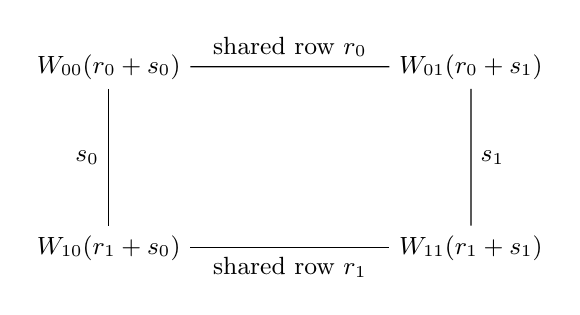
\begin{tikzpicture}[every node/.style={font=\small},scale=1.15]
\node (a) at (0,2) {$W_{00}(r_0+s_0)$};
\node (b) at (4,2) {$W_{01}(r_0+s_1)$};
\node (c) at (0,0) {$W_{10}(r_1+s_0)$};
\node (d) at (4,0) {$W_{11}(r_1+s_1)$};
\draw (a) -- node[above] {shared row $r_0$} (b);
\draw (c) -- node[below] {shared row $r_1$} (d);
\draw (a) -- node[left] {$s_0$} (c);
\draw (b) -- node[right] {$s_1$} (d);
\end{tikzpicture}
